
\chapter{Design of Blockchain-Based Voting Architecture}

Secure and anonymous electronic voting demands a careful separation between identity verification and vote recording. This chapter presents the architectural components of the proposed system and traces the end-to-end flow through which voter privacy is preserved. The design rationale for off-chain batching, identity hashing, and local blockchain deployment is elaborated across the following sections. Together, these elements form a modular pipeline that achieves anonymity without sacrificing auditability.

\section{System Overview}

The proposed system is composed of four principal layers: a voter-facing \gls{ui}, an off-chain batching and shuffle module, a relayer service, and an on-chain smart contract responsible for tallying. Voters authenticate at the \gls{ui}, select a candidate, and submit a vote that enters an off-chain buffer rather than being written directly to the chain. This buffering strategy is central to the privacy model — votes accumulate until a threshold batch size is reached, at which point they are shuffled and submitted in two distinct stages. By ensuring that hashed identities are marked used in one transaction and anonymized candidate \glspl{id} are recorded in a separate transaction, the system prevents any direct on-chain pairing of a voter to a choice.

\subsection{Voter Interface}

The \gls{ui} layer provides two interaction modes. The standard interface presents the ballot visually, allowing voters to select a candidate and confirm their submission through conventional controls. The voice-guided agentic interface targets voters who require assistance, offering a step-by-step spoken flow with explicit confirmation gates at each stage to prevent accidental submission. Both interfaces share the same underlying authentication and submission pipeline, ensuring consistent privacy properties regardless of the mode used.

\subsection{Off-Chain Buffer and Shuffle Module}

The off-chain buffer temporarily holds incoming votes as (hashed identity, candidate \gls{id}) pairs. Once the buffer accumulates a configurable threshold of entries, the module applies a shuffle to the list of candidate \glspl{id}, decoupling their ordering from the order in which votes were cast. This shuffle is the primary mechanism for breaking timing correlations that could otherwise allow an observer to infer which voter chose which candidate by comparing submission timestamps.

\subsection{Relayer Service}

The relayer is the sole actor authorized to submit batched transactions to the smart contract. It receives the shuffled batch from the off-chain module and performs a two-stage submission: first it forwards the array of hashed identities to mark them as used, and then it forwards the array of anonymized candidate \glspl{id} to update the tally. This separation into two transactions is a deliberate design choice — even if both transactions are visible on-chain, the shuffle ensures no positional correspondence exists between the two arrays.

\subsection{Smart Contract}

The smart contract enforces election lifecycle phases (registration, voting, closed), validates submitted candidate \glspl{id} against a declared candidate list, rejects any hashed identity that has already been marked as used, and maintains running candidate tallies. All state transitions are recorded immutably on the local chain. The contract exposes a read-only results function that returns aggregate counts without any per-voter data, supporting public auditability while preserving individual anonymity.

\section{System Flow Description}
\subsubsection{\textbf{Authentication and Identity Hashing}}
\begin{figure}[htbp]
    \centering
    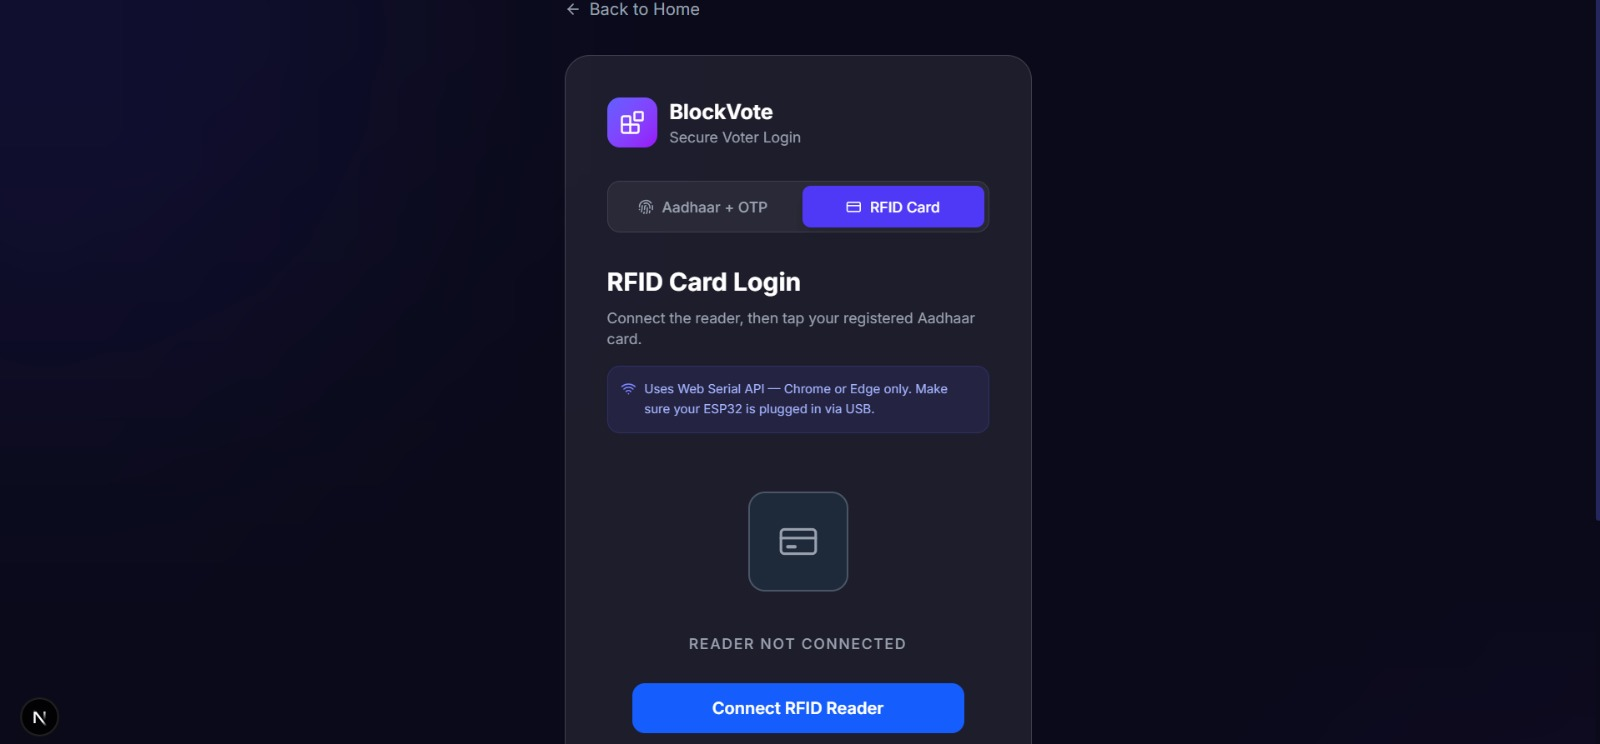
\includegraphics[width=0.8\linewidth]{Chapter2/2.2(1).jpeg}
    \caption{Authentication and Identity Hashing}
    \label{fig:Authentication and Identity Hashing}
\end{figure}


When a voter initiates a session, the \gls{ui} collects the identity credential and immediately computes a deterministic hash. The raw credential is discarded after hashing and is never stored, transmitted, or written to any persistent medium. The hash is used solely to verify eligibility and, once the vote is submitted, to mark the voter as having participated.

\subsubsection{\textbf{Candidate Selection}}

Following authentication, the voter selects a candidate. In the standard interface, selection is made via a visual ballot control. In the voice-guided flow, the system reads out candidate names and awaits a spoken or keyed confirmation at each decision point. A final confirmation gate is presented in both modes before the vote is committed to the buffer.

\subsubsection{\textbf{Buffering and Shuffle}}

The confirmed (hashed identity, candidate \gls{id}) pair is appended to the off-chain buffer. The buffer continues to accept incoming votes until its threshold is reached. At threshold, the candidate \gls{id} array is shuffled independently of the identity array. This shuffle is applied only to the candidate column; the identity column retains its original order for the first-stage submission. After the shuffle, the two arrays no longer share a meaningful positional mapping.
\begin{figure}[htbp]
    \centering
    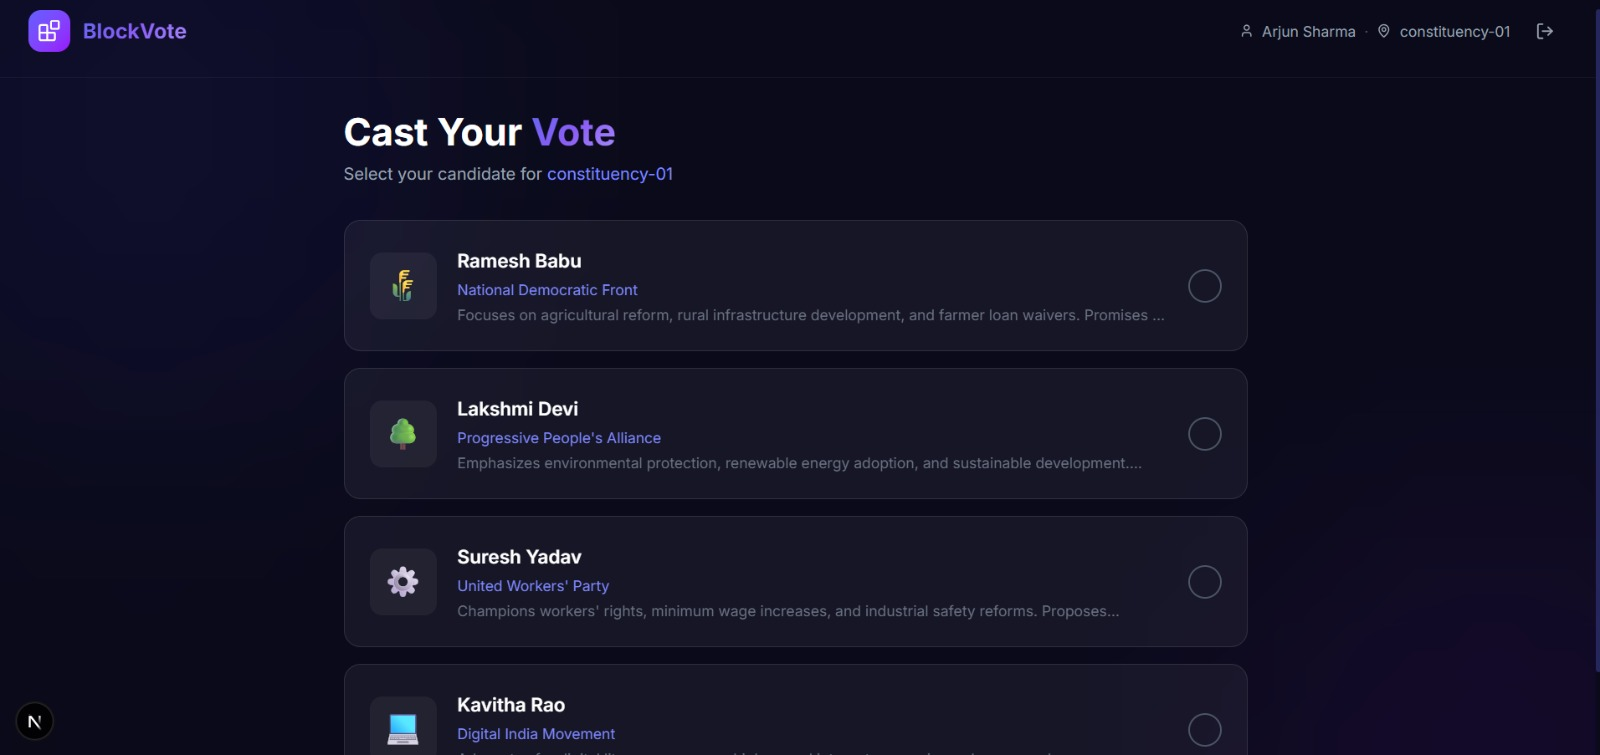
\includegraphics[width=0.8\linewidth]{Chapter2/2.2(2).jpeg}
    \caption{Candidate Selection}
    \label{fig:Candidate Selection}
\end{figure}

\subsubsection{\textbf{Two-Stage On-Chain Submission}}

The relayer submits the identity array to the smart contract in the first transaction, which marks each hash as used and enforces the no-double-vote constraint. The relayer then submits the shuffled candidate \gls{id} array in a second transaction, which increments the corresponding tally counters. Because the two transactions carry independently ordered arrays, no on-chain observer can reconstruct which identity corresponded to which candidate selection.

\section{Data Handling and Privacy}

Raw identity data is never retained beyond the hashing step. The off-chain buffer holds only hashed identities and candidate \glspl{id}, and both are discarded once the batch has been successfully submitted to the chain. On-chain state consists exclusively of a set of used identity hashes and a mapping of candidate \glspl{id} to vote counts. No per-vote record, timestamp, or sequence number that could enable re-identification is written to the ledger.

\subsection{Threat Model Considerations}

The design addresses two primary threat classes. The first is linkage attack: an adversary attempts to pair a voter identity with a candidate choice by correlating on-chain data. The shuffle step and the two-stage submission together eliminate the positional mapping required for this attack. The second is double-vote fraud: a voter or a compromised relayer attempts to register more than one vote for the same identity. The smart contract's duplicate-rejection logic defeats this by treating the identity hash set as a spent-key register.

\subsection{Local Blockchain Rationale}

Deployment on a local (private) chain rather than a public network provides two practical benefits. First, it removes the dependency on external validators and network fees, making the system viable for edge environments with limited or intermittent connectivity. Second, it constrains the visible surface of on-chain data to participants within the deployment boundary, reducing exposure to passive chain analysis. The modular architecture is designed so that migration to a public or permissioned chain in a future phase requires changes only to the deployment configuration, not to the application logic.

\section{Tools and Technologies Used}

\subsection{Smart Contract Platform}

The smart contract is implemented in Solidity and deployed to a local \gls{evm}-compatible chain. A local node instance provides the \gls{rpc} endpoint consumed by the relayer. This setup allows the full contract lifecycle — deployment, interaction, and state inspection — to be exercised without external dependencies.

\subsection{Off-Chain Components}

The off-chain buffer, shuffle module, and relayer are implemented as a lightweight service with a \gls{rest} interface. The service maintains buffer state in memory and exposes endpoints for vote submission (called by the \gls{ui}) and batch flush (triggered internally at threshold). The shuffle algorithm uses a cryptographically seeded Fisher-Yates permutation to ensure unpredictability of the resulting order.

\subsection{User Interface Framework}

The standard \gls{ui} is built as a web-based single-page application. The voice-guided interface uses a browser-native speech \gls{api} for output and a text input fallback for environments where speech recognition is unavailable. Both interfaces communicate with the off-chain service over \gls{https}.
\begin{figure}[htbp]
    \centering
    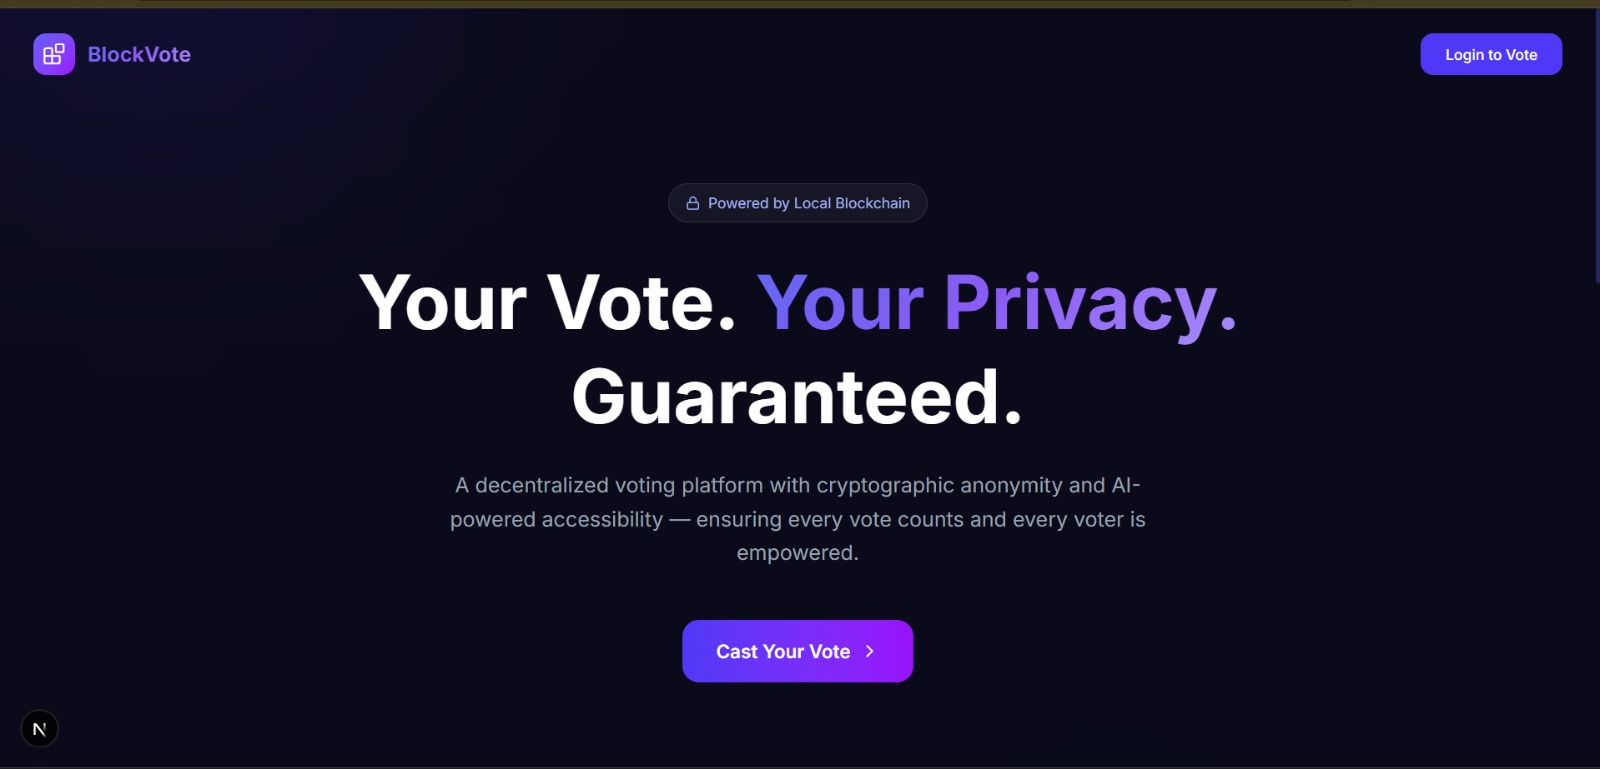
\includegraphics[width=0.8\linewidth]{Chapter2/2.jpeg}
    \caption{Standard Visual Interface}
    \label{fig:voter interface 1}
\end{figure}
\begin{figure}[htbp]
    \centering
    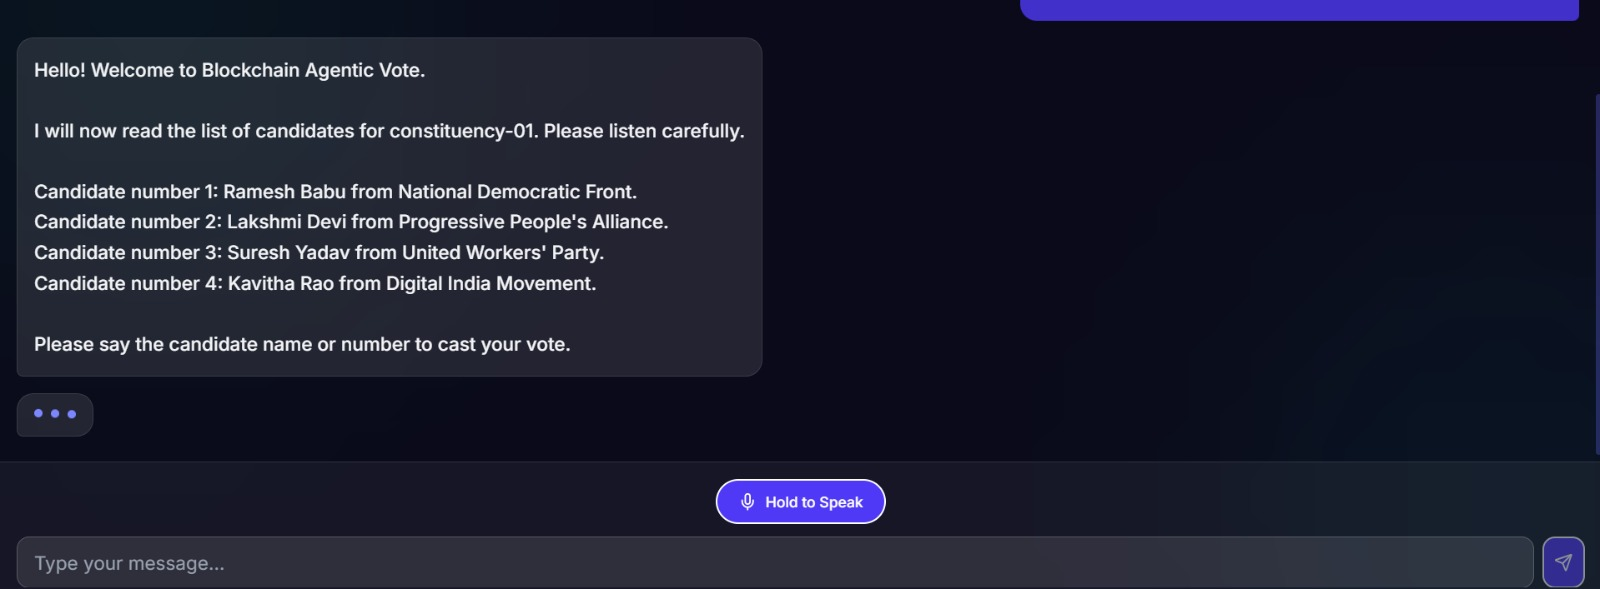
\includegraphics[width=0.8\linewidth]{Chapter2/2.2.jpeg}
    \caption{Voice-Guided Interface}
    \label{fig:voter interface 2}
\end{figure}

\section{Use of Acronyms and Glossaries}

Acronyms used throughout this report are defined at first use and thereafter appear in their short form. For example, \gls{ui}, \gls{evm}, \gls{rpc}, \gls{rest}, and \gls{api} are defined in the \texttt{Glossaries.tex} file and referenced using \verb|\gls{<Ref>}|. The first occurrence of each acronym expands to its full form with the abbreviation in parentheses; subsequent occurrences show only the abbreviation. All acronym definitions follow the syntax:

\begin{verbatim}
%\newacronym{<Ref>}{<Short-Form>}{<Expanded word>}
\newacronym{ui}{UI}{User Interface}
\newacronym{evm}{EVM}{Ethereum Virtual Machine}
\newacronym{rpc}{RPC}{Remote Procedure Call}
\newacronym{rest}{REST}{Representational State Transfer}
\newacronym{api}{API}{Application Programming Interface}
\end{verbatim}

This chapter has presented the full system architecture of the proposed blockchain-based voting system, covering the \gls{ui} layer, off-chain batching and shuffle pipeline, relayer service, and on-chain smart contract. The two-stage submission model and the local-chain deployment strategy together address the core requirements of voter anonymity and result auditability without reliance on centralized infrastructure. The following chapter details the implementation of each component, describing the specific code structure, contract functions, and the interface flows for both standard and voice-guided voting modes.

